\newpage

\section{Le correcteur orthographique}
Nous aurions pus utiliser sur le texte le correcteur orthographique de GTK mais nous nous sommes quand meme interesser a la correction orthographique suivant deux methodes 
\subsection{Les arbres lexicaux}
Pour detecter les mots qui ne sont pas valides dans un  texte nous utilisons une structure d'arbre lexicaux 
\begin{center}
	\begin{figure}[h]
		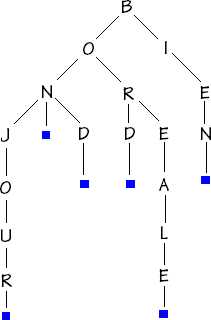
\includegraphics{arbre17.png}
		\caption{schema d'un arbre lexical pour la lettre B}
	\end{figure}
\end{center}
Ce schema resume bien la construction d'un tel ensemble.\\
Pour verifier l'existance d'un mot il ne reste plus qu'a parcourir l'arbre dont la racine correspond a la premiere lettre de notre mot.
Nous executons alors ca sur tout les mots de notre texte et nous creeons ainsi un liste de mots qui n'existe pas.\\
Une fois notre liste complete, les deux methodes suivantes vont nous permettres de creer une liste de mots qui peuvent remplacer nos faux mots.
\subsection{La distance de levenshtein}
La distanve de levenshtein se base sur la difference de suppresion addition et substitution de lettre entre deux mots. Cette methode se base sur le calcul d'une matrice entre les deux mots. 
\subsubsection{Petite histoire}
Elle fut creer en 1965 par Vladimir Levenshtein.
\subsubsection{L'algorithme}
L'algortihme prends en parametre deux chaines de caracteres. Il va pour chaque caractere dela chaine 1 parcourir la chaine 2. Si deux characteres sont egaux alors le cout entre les 2 est de 0 sinon il vaut 1. On va ainsi creer une matrice dont les cases suivront cette formule : 
\[m[i,j] = Min ( m[i-1,j] + 1, m[i,j+1] + 1, m[i-1,j-1] + cout)\]
Nous avons choisis une valeur de 2 pour le cout.
Voila un exemple de matrice obtenue grace a levenshtein :
\begin{center}
		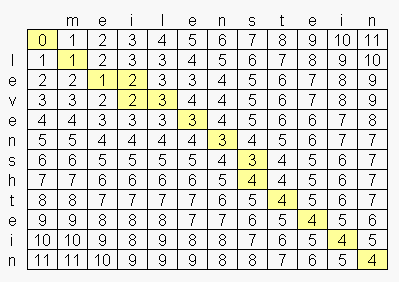
\includegraphics{Levenshtein-Distance_2.png}
\end{center}
La distance de levenshtein enter levenshtein et meilenstein vaut 4 (lecture en bas a droite de la matrice).

\subsection{Soundex}
L'algorithme soundex se base sur la phonetique du mots, il en existe donc plusieur version suivant la langue. Nous avons donc choisis d'en implementer un en francais.
\subsubsection{Petite histoire}
Soundex a ete cree par Robert Russel et margaret Odell en 1918 et fut d'ecrit par Donald knuth dans "the art of computer programming"
\subsubsection{L'algorithme}
Nous prenons notre mots et nous allons lui faire subir plusieur transformation.
\begin{itemize}
	\item Passage en majuscule.
	\item On conserve la premiere lettre du mot 
	\item on supprime ensuite tout les lettres tel que: a, e, h, i, o, u, w, y.
	\item on associe ensuite a chaquer lettre une valeur comme suit :
		\begin{enumerate}
		\item = b, f
		\item = c, k, q
		\item = d, t
		\item = l
		\item = m, n
		\item = r
		\item = g, j
		\item = x, z, s
		\item = f, v
		\end{enumerate}
	      \item un fois que l'on attribuer a chaque lettre restante on en garde que 3 et ca nous forme le "code" soundex du mots.
\end{itemize}

voila quelque exemple de résultats de soundex : 
\begin{itemize}
  \item Krisboul = K681
  \item Clafoutis = C413
\end{itemize}
\subsection{Ce qui n'a pas marcher}
L'implementation des deux algorithmes n'était surement pas assez précise nous obtenons des resultats mais pas suffisament precis. Il faudrait revoir l'association des deux algorithmes.
